\section{Evaluation}
\label{sec:Evaluation}
%______________________________________________________________________

\subsection{General Information}
\label{subsec:GeneralInformation}
%______________________________________________________________________

\subsubsection{RQ1: Publisher}
\label{subsubsec:RQ1}
As defined in the chapter \ref{subsubsec:general_information}, the first research question is:
\begin{displayquote}
\textbf{RQ1) }\quoteit{Who published the paper?}
\end{displayquote}
For the selected papers (see the section \ref{subsubsec:selected_papers}), 9 different publishers could be distinguished. 
\begin{table}[!ht]
\begin{center}
\begin{tabular}{ |p{7cm}|c| }
	\hline
 	Publisher & Publication(s) \\ [0.5ex] 
 	\hline\hline
 		IEEE  & \cite{2015_Zyskind,2017_Gipp,2016_Kianmajd,2016_Yasin,2015_Dennis,2016_Azaria,2016_Tian} \\ 
	 \hline
	 Springer & \cite{2017_Tackmann,2016_Schaub,2016_Jacynycz,2016_Sharples,2017_Jaag,2017_Ouaddah,2016_Yue} \\  
	 \hline
	 AIS Electronic Library (AISeL) & \cite{2017_Madhwal,2017_Naerland} \\ 
	 \hline
	 American Accounting Association (AAA) & \cite{2017_Coyne} \\  
	 \hline
	 arXiv.org & \cite{2018_Lucena} \\  
	 \hline
	 Indonesian Society for Knowledge and Human Development (INSIGHT) & \cite{2018_Alessandra} \\
	 \hline
	 Scientific Research Publishing (SCIRP) & \cite{2016_Bahga} \\ 
	 \hline
	 University of Calgary (U of C) & \cite{2017_Liu} \\ 
	 \hline
\end{tabular}
\end{center}
\caption{Publishers} \label{tab:rq1_publisher}
\end{table}
\paragraph{IEEE} \enquote{IEEE}\footnote{\url{https://www.ieee.org/}} is globally the biggest organization committed to encourage the progress of technology. They have more than 423,000 members in over 160 countries. They provide publications in the domains of engineering, computing, and technology information.
\paragraph{Springer}
Springer \footnote{\url{https://www.springer.com/}} is a worldwide publishing firm that issues books, e-books and journals in areas like science, humanities, and many more.
\quoteit{SpringerLink}\footnote{\url{https://link.springer.com/}} is a online scientific database provided by Springer that holds a collection of journals, books and other publications.
\paragraph{American Accounting Association (AAA)} Founded in 1916, the AAA\footnote{\url{http://aaahq.org}} is the largest association for accountants in the academic field. Their focus lies on teaching, researching, publishing and keeping a constant network for accountants.
\paragraph{arXiv.org} \quoteit{arXiv.org}\footnote{\url{https://arxiv.org}} is an online archive for research publications that was founded in 1991. It provides open access to articles in the areas of physics, mathematics, computer science, nonlinear sciences, quantitative biology, quantitative finance, statistics, electrical engineering and systems science, and economics, and also the opportunity to submit own research. The archive is managed by the Cornell University Library.
\paragraph{Indonesian Society for Knowledge and Human Development (INSIGHT)} \quoteit{INSIGHT}\footnote{\url{http://www.insightsociety.org/}} is an association of experts from all technology, science and engineering practices. They produce the \quoteit{International Journal on Advanced Science, Engineering and Information Technology}\urlfootnote{http://ijaseit.insightsociety.org/}.
\paragraph{Scientific Research Publishing (SCIRP)} \quoteit{SCIRP}\footnote{\url{https://www.scirp.org}} is also an open-access online repository for research articles and journals. It includes a broad range of areas, like biomedical \& life sciences, business \& economis, chemistry \& materials science, computer sciences \& communications and many more.
\paragraph{AIS Electronic Library (AISeL)} The \quoteit{AISeL}\footnote{\url{http://aisel.aisnet.org/}} was founded by the Association for Information Systems (AIS) and is an online archive for research papers and journal articles that focus on information systems. It includes publications of the \quoteit{International Conference on Information Systems (ICIS)} and the \quoteit{Americas Conference on Information Systems (AMCIS)}, as well as all other publication channels related to the subject.
\paragraph{University of Calgary (U of C)} The \quoteit{U of C}\footnote{\url{https://www.ucalgary.ca/}} is a public univeristy in Canada. They provide open-access to certain research papers on their website.

\begin{figure}[!ht]
	\centering
	\begin{tikzpicture}
		\pie[sum=21,text=legend]{7/Springer , 7/IEEE ,2/AISeL , 1/AAA , 1/UoC,  1/SCIRP , 1/INSIGHT , 1/arXiv.org } 
	\end{tikzpicture}
	\caption{Number of publications per publisher} 	
	\label{graph:rq1_publishers}
\end{figure}


%______________________________________________________________________

\clearpage
\subsubsection{RQ2: Publication Type }
\label{subsubsec:rQ2_publication_type}
As defined in the chapter \ref{subsubsec:general_information}, the second research question is:
\begin{displayquote}
\textbf{RQ2) }\quoteit{What was the publication type of the paper?}
\end{displayquote}
For the selected papers (see the section \ref{subsubsec:selected_papers}), three (see figure \ref{tab:rq2_publication_type}) different publication types could be identified.
\begin{longtable}{ |c|c| }
	\caption{Publication Types} \label{tab:rq2_publication_type}  \\
	\hline
 	Publication Type & Publication(s) \\ [0.5ex] 
 	\hline\hline
 		Inproceedings  & \cite{2016_Azaria,2015_Dennis,2017_Gipp,2016_Jacynycz,2016_Kianmajd,2017_Naerland,2017_Ouaddah, 2016_Schaub,2017_Tackmann,2016_Sharples,2016_Tian,2016_Yasin,2015_Zyskind} \\ 
	 \hline
	 Article & \cite{2018_Alessandra,2016_Bahga,2017_Coyne,2017_Liu,2018_Lucena,2017_Madhwal,2016_Yue} \\  
	 \hline
	 InBook & \cite{2017_Jaag} \\  
	 \hline
\end{longtable}
There are various types of scientific papers. In this synthesis, the ones that are provided by \textsc{Bib}\TeX \footnote{\url{http://www.bibtex.org/}} are used. \textsc{Bib}\TeX is a reference management software. It is mostly used to create lists of references for the document preparation system \LaTeX. The types are\footnote{\url{https://en.wikipedia.org/wiki/BibTeX}}
\begin{itemize}[noitemsep]
	\item \textit{Article:} An article that was published in a journal or magazine
	\item \textit{Book:} A book (with a publisher)
	\item \textit{Booklet:} A published work without a reference to the publisher 
	\item \textit{InBook:} A part of a book 
	\item \textit{InCollection:} A part of a book with an explicit title
	\item \textit{Inproceedings:} An article that was presented in the context of a conference proceeding 
	\item \textit{Manual:} A technical documentation 
	\item \textit{Mastersthesis:} A master’s thesis
	\item \textit{Misc:} If no other type fits your resource, use this one 
	\item \textit{Phdthesis:} A Ph.D. thesis 
	\item \textit{Proceedings:} Collection of scientific papers that were published during a conference 
	\item \textit{Techreport:} A report (usually published by a school/university) 
	\item \textit{Unpublished:} A document that has not been officially published
\end{itemize}
\begin{figure}[!ht]
	\centering
	\begin{tikzpicture}
		\pie[sum=21,text=legend]{13/Inproceedings , 7/Article , 1/InBook} 
	\end{tikzpicture}
	\caption{Number of publications per publication type} 	
	\label{graph:rq2_publication_type}
\end{figure}


%______________________________________________________________________
\clearpage

\subsubsection{RQ3: Publication Channel}
\label{subsubsec:rq3_publication_channel}
As defined in the chapter \ref{subsubsec:general_information}, the third research question is:
\begin{displayquote}
\textbf{RQ3) }\quoteit{Where was the paper published?}
\end{displayquote}
For the selected papers (see the section \ref{subsubsec:selected_papers}), 19 different publication channels could be identified. For one article, no information was provided.\\
\begin{longtable}{ |p{5cm}|c|c| }
\caption{Publication Channels} \label{my_label}\\
	\hline
 	Publication Channel & Rating &  Publication(s) \\ [0.5ex] 
 	\hline\hline
	 Joint Conference on Digital Libraries (JCDL) \nomenclature[P]{JCDL}{Joint Conference on Digital Libraries} & A* & \citet{2017_Gipp} \\ 
	 \hline
	 IEEE International Conference on Computer Communications (IEEE INFOCOM) \nomenclature[P]{IEEE INFOCOM}{IEEE International Conference on Computer Communications} & A* & \citet{2016_Kianmajd} \\ 
	 \hline
	 International Conference on Information Systems (ICIS) & A* & \citet{2017_Naerland} \\ 
	 \hline
	IEEE Symposium on Security and Privacy (S\&P)\nomenclature[P]{S\&P}{IEEE Symposium on Security and Privacy} & A* & \citet{2015_Zyskind} \\ 
	 \hline
 		Americas Conference on Information Systems (AMCIS)\nomenclature[P]{AMCIS}{Americas Conference on Information Systems}  & A & \citet{2017_Madhwal} \\ 
	 \hline
	 European Symposium On Research In Computer Security (ESORICS) \nomenclature[P]{ESORICS}{European Symposium On Research In Computer Security} & A & \citet{2017_Tackmann} \\ 
	 \hline
	 IFIP Information Security \& Privacy Conference (IFIP SEC) \nomenclature[P]{IFIP SEC}{IFIP Information Security \& Privacy Conference}& B & \citet{2016_Schaub} \\
	 \hline
	 International Computer Software and Applications Conference (COMPSAC)\nomenclature[P]{COMPSAC}{International Computer Software and Applications Conference}  & B & \citet{2016_Yasin} \\ 
	 \hline
	 Journal of Medical Systems & C & \citet{2016_Yue} \\ 
	 \hline
	 Journal of Software Engineering and Applications (JSEA) \nomenclature[P]{JSEA}{Journal of Software Engineering and Applications}  & Not ranked & \citet{2016_Bahga} \\ 
	 \hline
	 International Journal on Advanced Science, Engineering and Information Technology (IJASEIT) \nomenclature[P]{IJASEIT}{International Journal on Advanced Science, Engineering and Information Technology} & N\textbackslash A & \citet{2018_Alessandra} \\ 
	 \hline
	 International Conference on Open and Big Data (OBD) \nomenclature[P]{OBD}{International Conference on Open and Big Data} & N\textbackslash A & \citet{2016_Azaria} \\ 
	 \hline
	 Journal of Emerging Technologies in Accounting (JETA)\nomenclature[P]{JETA}{Journal of Emerging Technologies in Accounting} & N\textbackslash A & \citet{2017_Coyne} \\ 
	 \hline
	 International Conference for Internet Technology and Secured Transactions (ICITST)\nomenclature[P]{ICITST}{International Conference for Internet Technology and Secured Transactions}& N\textbackslash A & \citet{2015_Dennis} \\ 
	 \hline
	 Book \enquote{The Changing Postal and Delivery Sector} & N\textbackslash A & \citet{2017_Jaag} \\ 
	 \hline
	 International Conference on Distributed Computing and Artificial Intelligence (DCAI)\nomenclature[P]{DCAI}{International Conference on Distributed Computing and Artificial Intelligence} & N\textbackslash A & \citet{2016_Jacynycz} \\ 
	 \hline
	 N\textbackslash A & N\textbackslash A & \citet{2017_Liu} \\ 
	 \hline
	Symposium on Foundations and Applications of Blockchain (FAB) \nomenclature[P]{FAB}{Symposium on Foundations and Applications of Blockchain} & N\textbackslash A & \citet{2018_Lucena} \\ 
	 \hline
	 Book \enquote{Europe and MENA Cooperation Advances in Information and Communication Technologies} & N\textbackslash A & \citet{2017_Ouaddah} \\ 
	 \hline
	 European Conference on Technology Enhanced Learning (EC-TEL)\nomenclature[P]{EC-TEL}{European Conference on Technology Enhanced Learning} & N\textbackslash A & \citet{2016_Sharples} \\ 
	 \hline
	 International Conference on Service Systems and Service Management (ICSSSM)\nomenclature[P]{ICSSSM}{International Conference on Service Systems and Service Management} & N\textbackslash A & \citet{2016_Tian} \\ 
	 \hline
\end{longtable}
\paragraph{Joint Conference on Digital Libraries (JCDL)}
The JCDL\footnote{\url{http://www.jcdl.org/}} is a combination of the ACM Digital Libraries Conference and the IEEE-CS Advances in Digiitales libraries Conference.
The core research suject are the technical, practical and social problems of digital libraries. The conference was ranked with an A*\footnote{\url{http://portal.core.edu.au/conf-ranks/2085/}}.
\paragraph{IEEE International Conference on Computer Communications (IEEE INFOCOM)} The \quoteit{IEEE INFOCOM}\footnote{\url{https://ieeexplore.ieee.org/xpl/conhome.jsp?punumber=1000359}} is focused on the theoretical and systems research in the domain of networking. It is an annual forum that started in 1982. The conference was ranked with an A* \footnote{\url{http://portal.core.edu.au/conf-ranks/2074/}}.
\paragraph{International Conference on Information Systems (ICIS)}
The \quoteit{ICIS}\urlfootnote{https://aisnet.org/page/ICISPage} is all about information systems. Starting in 1980, this conference is a annual flagship event that brings together academics and researchers in this area. The conference was ranked with an A*\urlfootnote{http://portal.core.edu.au/conf-ranks/1078/}. 
\paragraph{IEEE Symposium on Security and Privacy (S\&P)}
The \quoteit{IEEE (S\&P)}\footnote{\url{https://ieeexplore.ieee.org/xpl/conhome.jsp?punumber=1000646}} is a yearly symposium that has been held since 1980. Its research focus is on computer security and electronic privacy. The conference was ranked with an A*\footnote{\url{http://portal.core.edu.au/conf-ranks/750/}}.
\paragraph{Americas Conference on Information Systems (AMCIS)} The \quoteit{AMCIS}\footnote{\url{http://aisel.aisnet.org/amcis/}} is a yearly conference since 1995. The papers presented at this conference talk about the areas information systems and information technology. The conference was ranked with an A\footnote{\url{http://portal.core.edu.au/conf-ranks/115/}}.
\paragraph{European Symposium On Research In Computer Security (ESORICS)}
Being held for the first time in 1990, \quoteit{ESORICS}\footnote{\url{http://conf.laas.fr/esorics/}} is a conference on computer, information and cyber security and privacy. Their goal was also to create a european forum that brings together different researches in the area. The conference was ranked with an A\footnote{\url{http://portal.core.edu.au/conf-ranks/515/}}.
\paragraph{IFIP Information Security \& Privacy Conference (IFIP SEC)} The \quoteit{IFIP SEC}\footnote{\url{https://www.ifipsec.org/}} is an event that focuses on information processing systems, especially on the information security and privacy protection. It is the most important event of the International Federation for Information Processing Technical Committee. The first conference was in 1986. The conference was ranked with a B\footnote{\url{http://portal.core.edu.au/conf-ranks/804/}}.
\paragraph{International Computer Software and Applications Conference (COMPSAC)}
The research focus in the \quoteit{COMPSAC}\urlfootnote{https://ieeexplore.ieee.org/xpl/conhome.jsp?punumber=1000143} is on computer and software technologies and applications. It is a forum for researchers to talk about research, progress, open questions and future trends in the area. The conference was ranked with a B\footnote{\url{http://portal.core.edu.au/conf-ranks/871/}}.
\paragraph{Journal of Medical Systems}
The Journal of Medical Systems\urlfootnote{https://link.springer.com/journal/10916} is published by Springer. It publishes various articles that talk about information systems in health care. The journal includes six different sections:
\begin{itemize}[noitemsep]
	\item Mobile \& Wireless Health
	\item Quality Improvement
	\item Transaction Processing Systems
	\item Image \& Signal Processing
	\item Patient Facing Systems
	\item Education \& Training
\end{itemize}
The journal was ranked with a C\urlfootnote{http://portal.core.edu.au/jnl-ranks/615/}.
\paragraph{Journal of Software Engineering and Applications (JSEA)}
The \quoteit{JSEA}\urlfootnote{http://www.scirp.org/journal/JournalArticles.aspx?JournalID=45} is a journal on software engineering and application. The aim of the journal is to provide a forum for academicians world-wide to improve, share and argues about new concerns and developments in the field.
The journal was ranked with \quoteit{Not ranked}\urlfootnote{http://portal.core.edu.au/jnl-ranks/413/}.
\paragraph{International Journal on Advanced Science, Engineering and Information Technology (IJASEIT)} The \quoteit{IJASEIT}\urlfootnote{http://ijaseit.insightsociety.org/} is an international journal. They publish articles related to all research in science, engineering and information technology. The journal was not ranked.
\nomenclature[O]{IT}{Information Technology}
\paragraph{International Conference on Open and Big Data (OBD)} The goal of the \quoteit{OBD}\urlfootnote{http://easyconferences.eu/portfolio/obd-2016/} conference is to analyze the combination of open data and big data. It is sponsored by the Technical Committee on the Internet of the IEEE Computer Socicety. The conference was not ranked.
\paragraph{Journal of Emerging Technologies in Accounting (JETA)}
The \quoteit{JETA}\urlfootnote{http://aaajournals.org/loi/jeta?code=aaan-site} is an academic journal that cover three domains
\begin{enumerate*}[label={\Alph*)},font={\color{red!50!black}\bfseries}]
	\item information technology
	\item accounting
	\item management advisory systems
\end{enumerate*}. 
Their goal is to promote and simplify the research, education and practice of information systems, new technologies and artificial intelligence (AI). The journal was not ranked.
\nomenclature[O]{AI}{Artificial intelligence}
\paragraph{International Conference for Internet Technology and Secured Transactions (ICITST)} The \quoteit{ICITST}\urlfootnote{http://icitst.org/} is an international refereed conference dedicated to the advancement of theory and practical implementation of secured internet transactions and to fostering discussions on the evolution of information technology. The conference was not ranked.
\paragraph{The Changing Postal and Delivery Sector} The book \quoteit{The Changing Postal and Delivery Sector}\urlfootnote{https://www.springer.com/gp/book/9783319460451} is about the important problems in postal and delivery services world-wide, in particular the dangers and chances of the digital competition. The book was not ranked.
\paragraph{International Conference on Distributed Computing and Artificial Intelligence (DCAI)} The \quoteit{DCAI}\urlfootnote{https://www.dcai-conference.net/} concentrates on distributed computing and artificial intelligence and their various application areas. The conference was not ranked.
\paragraph{Symposium on Foundations and Applications of Blockchain (FAB)} The one day symposium \quoteit{FAB}\urlfootnote{https://scfab.github.io/2018/} is about various aspects of the blockchain technology. Subjects that are being discussed are for example secure smart contracts and social aspects of blockchain. The symposium was not ranked.
\paragraph{Europe and MENA Cooperation Advances in Information and Communication Technologies} The book\urlfootnote{https://link.springer.com/book/10.1007/978-3-319-46568-5} contains the procceedings of the \quoteit{Europe, Middle East and North Africa Conference on Technology and Security to Support Learning 2016 (EMENA-TSSL'16)}. The field of interest is security to support learning and information \& communication technologies.
\nomenclature[O]{MENA}{Middle East and North Africa}
\nomenclature[P]{EMENA-TSSL}{Europe, Middle East and North Africa Conference on Technology and Security to Support Learning}
\paragraph{European Conference on Technology Enhanced Learning (EC-TEL)}
The \quoteit{EC-TEL}\urlfootnote{https://link.springer.com/conference/ectel} takes the imapct into account that technolgy has on learning methods and adresses ongoing challenges and advances in the field.
The conference was not ranked.
\paragraph{International Conference on Service Systems and Service Management (ICSSSM)} All fields related to information management are covered by th \quoteit{ICSSSM}\urlfootnote{https://ieeexplore.ieee.org/xpl/conhome.jsp?punumber=1002157} conference. The conference was not ranked.
\paragraph{Definitions} According to the \quoteit{Merriam-Webster Dictionary}\urlfootnote{https://www.merriam-webster.com/}, the following terms are defined as follows:
\begin{displayquote}
\textbf{Conference: }\quoteit{a meeting of two or more persons for discussing matters of common concern}
\end{displayquote}
\begin{displayquote}
\textbf{Symposium: }\quoteit{a formal meeting at which several specialists deliver short addresses on a topic or on related topics}
\end{displayquote}
\begin{displayquote}
\textbf{Journal: }\quoteit{a periodical dealing especially with matters of current interest}
\end{displayquote}
\begin{displayquote}
\textbf{Book: }\quoteit{something that yields knowledge or understanding}
\end{displayquote}

\begin{figure}[!ht]
	\centering
	
\begin{tikzpicture}
		\pie[sum=21,text=legend]{11/Conference , 3/Symposium , 4/Journal , 2/Book , 1/N\textbackslash A} 
	\end{tikzpicture}
	\caption{Ranking} \label{graph:rq3_publication_channel_1}
\end{figure}

\clearpage
\paragraph{CORE Rankings Portal }The \quoteit{Computing Research and Education Association of Australasia (CORE)} is a community of various computer science departements of different universities all over Australia and New Zealand. Their objectives are over all to 
\begin{enumerate*}[label={\Alph*)},font={\color{red!50!black}\bfseries}]
	\item create a professional community for computer scientists and information technologists
	\item aid and progress research and teaching in these areas
	\item present a forum open for discussion 
	\item encourage partnerships with other organizations
\end{enumerate*}. 
They provide the \quoteit{CORE Rankings Portal} on their website. 
The \quoteit{CORE Conference Ranking}\footnote{\url{http://portal.core.edu.au/conf-ranks/}} evaluates significant conferences in various computing disciplines and the \quoteit{CORE Journal Ranking}\footnote{\url{http://portal.core.edu.au/jnl-ranks/}} ranks different journals. The different ranks are:
\begin{itemize}[noitemsep]
	\item \textbf{A*} \quoteit{flagship conference}: an outstanding conference in its field
	\item \textbf{A} \quoteit{excellent conference}: a highly valued conference in its field
	\item \textbf{B} \quoteit{good conference}: a well valued conference in its field
	\item \textbf{C} \quoteit{other conference}: a confernce that satisfies minimal demands
	\item \textbf{Australasian} \quoteit{australasian conference}: a conference that is mainly in Australia and New Zealand
	\item \textbf{Unranked} \quoteit{unranked conference}: an unranked conference
	\item \textbf{National} \quoteit{national conference}: a conference that is mainly in one specific country
	\item \textbf{Regional} \quoteit{regional conference}: a conference that is mainly in one specific region
\end{itemize}
\begin{figure}[!ht]
	\centering
	
\begin{tikzpicture}
		\pie[sum=20,text=legend]{3/A* , 2/A , 2/B , 1/C , 1/Not ranked , 11/N\textbackslash A} 
	\end{tikzpicture}
	\caption{Ranking 1} \label{graph:rq3_publication_channel_1}
\end{figure}

%______________________________________________________________________

\clearpage
\subsubsection{RQ4: Publication Date}
\label{subsubsec:rq4_publication_date}
As defined in the chapter \ref{subsubsec:general_information}, the fourth research question is:
\begin{displayquote}
\textbf{RQ4) }\quoteit{When was the paper published?}
\end{displayquote}
As can be seen in figure \ref{tab:rq4_publication_date}, the selected papers (see the section \ref{subsubsec:selected_papers}) were all published between 2015 and 2018. \\
\begin{longtable}{ |c|c| }
	\caption{RQ4: Publication Date} \label{tab:rq4_publication_date} \\
	\hline
 	Publication Year & Publication(s) \\ [0.5ex] 
 	\hline\hline
 		2015  & \cite{2015_Dennis,2015_Zyskind} \\ 
	 \hline
	 2016 & \cite{2016_Azaria,2016_Bahga,2016_Jacynycz,2016_Kianmajd,2016_Schaub,2016_Sharples,2016_Tian,2016_Yasin,2016_Yue} \\  
	 \hline
	 2017 & \cite{2017_Coyne,2017_Gipp,2017_Jaag,2017_Liu,2017_Madhwal,2017_Naerland,2017_Ouaddah,2017_Tackmann} \\
	 \hline
	 2018 & \cite{2018_Alessandra,2018_Lucena} \\
	 \hline
\end{longtable}

\begin{figure}[!ht]
	\centering
	\begin{tikzpicture}
		\pie[sum=21,text=legend]{2/2015 , 9/2016 , 8/2017 , 2/2018} 
	\end{tikzpicture}
	\caption{Publication Date 1} \label{graph:rq4_publication_date_1}
\end{figure}

%______________________________________________________________________

\clearpage
\subsubsection{RQ5: Keywords}
\label{subsubsec:rq5_keywords}
As defined in the chapter \ref{subsubsec:general_information}, the fifth research question is:
\begin{displayquote}
\textbf{RQ5) }\quoteit{What kind of keywords were used?}
\end{displayquote}
From the twenty publications selected (see the section \ref{subsubsec:selected_papers}) three \cite{2017_Liu,2018_Lucena,2017_Tackmann} did not provide keywords, they were therefore excluded from this evalutation. This leaves a total of seventeen publications that stated keywords.
\begin{longtable}{ |c|p{9cm}| }
	\caption{Keywords} \\
	\hline
 	\textbf{Publication} & \textbf{Keywords} \\ [0.5ex] 
 	\hline\hline
 	\endhead
 	\citet{2018_Alessandra} & \textit{Information Technology, Smart City, Digital Revolution, Digital Innovation, Blockchain, Smart Energy Grid, Machine Learning}\\ 
	 \hline
	  \citet{2016_Azaria} & \textit{electronic medical records, cryptographic protocols, access control, distributed information systems} \\ 
	 \hline
	 \citet{2016_Bahga} & \textit{Internet of things, Blockchain, Smart Contracts, Cloud-based manufacturing}\\ 
	 \hline
	 \citet{2017_Coyne} & \textit{financial accounting, blockchain, ledger, database}\\ 
	 \hline
	 \citet{2015_Dennis} & \textit{Blockchain, reputation systems, cryptographic protocols, distrubted networks, peer-to-peer, Bittorent} \\ 
	 \hline
	 \citet{2017_Gipp} & \textit{Electronic publishing,
peer review, manuscript   submission, blockchain, conference management, scientific data managemet} \\ 
	 \hline
	 \citet{2017_Jaag} & \textit{Credit Card, Financial Service, Payment System, Financial Intermediary, Financial Inclusion } \\ 
	 \hline
	 \citet{2016_Jacynycz} & \textit{Bitcoin, Blockchain, Bounty, Crowdfunding, Cryptocurrencies, Distributed Software, Ethereum, P2P, Smart contract} \\ 
	 \hline
	 \citet{2016_Kianmajd} & \textit{Protocols, Power demand, Cryptography, Microgrids, Home appliances, Internet of Things, Schedules} \\ 
	 \hline
 		\citet{2017_Madhwal} & \textit{Supply Chain Management, Blockchain, Aircraft, Segments} \\ 
	 \hline
	 \citet{2017_Naerland} & \textit{Blockchain, Bill of Lading, International Trade, Decentralized Environments}\\
	 \hline
	 \citet{2017_Ouaddah} & \textit{Internet of things, Security, Privacy, Access control, Blockchain, Bitcoin, Cryptocurrency} \\ 
	 \hline
	 \citet{2016_Schaub} & \textit{Service Provider, Blind Signature, Certification Authority, Trusted Third Party, Reputation System} \\
	 \hline
	 \citet{2016_Sharples} & \textit{Blockchain, Reputation management, Self-determined learning, e-portfolios, Records of achievement} \\ 
	 \hline
	 \citet{2016_Tian} & \textit{Agri-food supply chain, traceability system, RFID, blockchain, food safety} \\ 
	 \hline
	 \citet{2016_Yasin} & \textit{Digital Identity, Online Reputation, Blockchain, Smart Contract Utility}\\ 
	 \hline
	\citet{2016_Yue} & \textit{Healthcare data system, Indicator-centric schema, BlockChain, Healthcare data sharing, Privacy Riks}\\ 
	 \hline
	 \citet{2015_Zyskind} & \textit{Blockchain, Privacy, Bitcoin, Personal data} \\ 
	 \hline
\end{longtable}


There are two kind of categories of keywords. The first are words that describe the technical content of the paper and the second are thos that explain the application area.
\begin{figure}[ht!]
\centering
\caption{Keywords} \label{fig:keywords_categories}
\begin{tikzpicture}
  % Blockchain Reviews
  \node[draw,fill=gray,text=white] (Keywords) at (0,0) {Keywords};
  \node[draw,fill=gray,text=white] (Technology) at (-2,-2) {Technology};
  \node[draw,fill=gray,text=white] (Application Area) at (2,-2) {Application Area};
  
  \draw node[vertex] (Joint) at (0,-0.25) {}; 
  \draw[->,draw=blue] (Joint) to (Technology);  
  \draw[->,draw=blue] (Joint) to (Application Area); ;   
  
\end{tikzpicture}
\end{figure}
\clearpage
All technical keywords that were found are listed in this table:
\begin{longtable}{ |c|c|p{4cm}| }
	\caption{Keywords} \\
	\hline
 	\textbf{Category} & \textbf{Term} & \textbf{Publication(s)} \\ [0.5ex] 
 	\hline\hline
 	\endhead
 	Bitcoin & Bitcoin & \cite{2016_Jacynycz,2017_Ouaddah,2015_Zyskind}\\ 
	 \hline
	 Blockchain & Blockchain & \cite{2018_Alessandra,2016_Bahga,2017_Coyne,2015_Dennis,2017_Gipp,2016_Jacynycz,2017_Madhwal,2017_Naerland,2017_Ouaddah,2016_Sharples,2016_Tian,2016_Yasin,2016_Yue,2015_Zyskind}\\ 
	 \hline
	 \multirow{3}{*}{Crypto} & cryptographic protocols & \cite{2016_Azaria,2015_Dennis} \\ \cline{2-3}
	 & Cryptocurrency(ies) & \cite{2016_Jacynycz,2017_Ouaddah}\\ \cline{2-3}
	 & Cryptography & \cite{2016_Kianmajd}\\
	 \hline
	  \multirow{3}{*}{Digital} & Digital Identity & \cite{2016_Yasin}\\ \cline{2-3}
	  & Digital Revolution & \multirow{2}{*}{\cite{2018_Alessandra}} \\ \cline{2-2}
	  & Digital Innovation & \\
	 \hline
	 \multirow{4}{*}{Distributed} & distributed networks & \cite{2015_Dennis}\\ \cline{2-3}
	  & distributed information systems
& \cite{2016_Azaria}\\ \cline{2-3}
	  & distributed software & \cite{2016_Jacynycz}\\ \cline{2-3}
	  & Decentralized environments & \cite{2017_Naerland} \\
	 \hline
 	Internet of Things & Internet of things & \cite{2016_Bahga,2017_Jaag,2016_Kianmajd}\\ 
	 \hline
	  \multirow{2}{*}{P2P} & peer-to-peer & \cite{2015_Dennis}\\ \cline{2-3} 
	  & P2P & \cite{2016_Jacynycz}\\
	 \hline
	 \multirow{2}{*}{Privacy} & Privacy & \cite{2017_Ouaddah,2015_Zyskind}\\  \cline{2-3}
	 & Privacy Risk & \cite{2016_Yue} \\
	 \hline
	 \multirow{2}{*}{Smart Contract} & Smart Contract(s) & \cite{2016_Bahga,2016_Jacynycz}\\ \cline{2-3}
	 & Smart Contract Utility & \cite{2016_Yasin} \\
	 \hline
	 \multirow{14}{*}{Others} & Bittorent  & \cite{2015_Dennis} \\ \cline{2-3}
	 & Bounty & \multirow{2}{*}{\cite{2016_Jacynycz}} \\ \cline{2-2}
	 & Ethereum & \\ \cline{2-3}
	 & Protocols & \cite{2016_Kianmajd} \\ \cline{2-3}
	 & Blind Signature & \multirow{3}{*}{\cite{2016_Schaub}} \\ \cline{2-2}
	 & Certification Authority & \\ \cline{2-2}
	 & Trusted Third Party & \\ \cline{2-3}
	 & Traceability system & \multirow{2}{*}{\cite{2016_Tian}} \\ \cline{2-2}
	 & RFID & \\ \cline{2-3}
	 & Indicator-centric schema & \cite{2016_Yue} \\ \cline{2-3}
	 & Ledger & \cite{2017_Coyne} \\ \cline{2-3}
	 & Security & \cite{2017_Ouaddah} \\ \cline{2-3}
	 & Information Technology & \multirow{2}{*}{\cite{2018_Alessandra}}\\ \cline{2-2}
	 & Machine Learning & \\
	 \hline
\end{longtable}
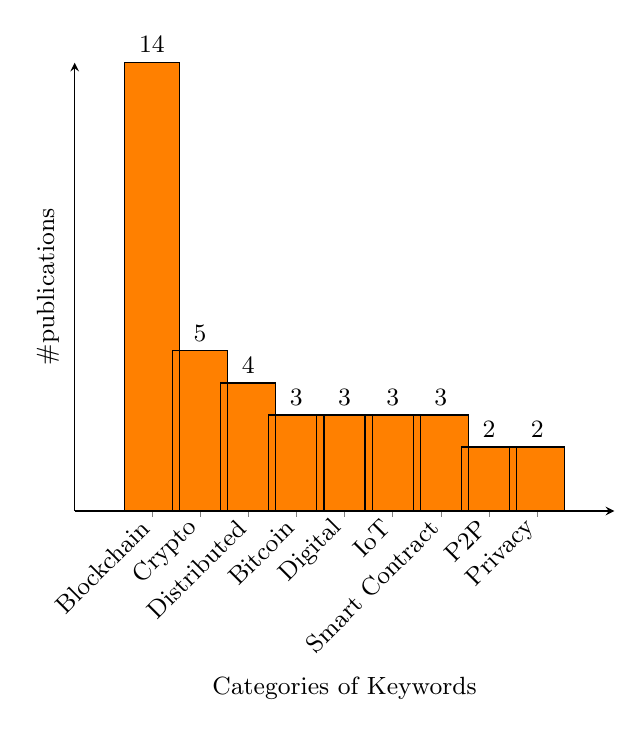
\begin{tikzpicture}[font=\small]
    \begin{axis}[
      ybar,
      bar width=20pt,
      xlabel={Categories of Keywords},
      ylabel={\#publications},
      ymin=0,
      ytick=\empty,
      xtick=data,
      axis x line=bottom,
      axis y line=left,
      enlarge x limits=0.2,
      symbolic x coords={Blockchain,Crypto,Distributed,Bitcoin,Digital,IoT,Smart Contract,P2P,Privacy},
      nodes near coords,
      xticklabel style={rotate=45,anchor=east},
    ]
      \addplot[fill=orange] coordinates {
        (Blockchain,14)
        (Crypto,5)
        (Distributed,4)
        (Bitcoin,3)
        (Digital,3)
        (IoT,3)
        (Smart Contract,3)
        (P2P,2)
        (Privacy,2)
      };
    \end{axis}
  \end{tikzpicture}

\clearpage
All keywords related to the application area can be found in this table:
\begin{longtable}{ |c|c|p{4cm}| }
	\caption{Keywords Application Area} \\
	\hline
 	\textbf{Category} & \textbf{Term} & \textbf{Publication(s)} \\ [0.5ex] 
 	\hline\hline
 	\endhead
 	Access control & Access control & \cite{2016_Azaria,2017_Ouaddah}\\ 
	 \hline
	 \multirow{7}{*}{Data/records} & Personal data & \cite{2015_Zyskind} \\  \cline{2-3}
	 & Electronic medical records & \cite{2016_Azaria} \\ \cline{2-3}
	 & Records of achievement & \cite{2016_Sharples} \\ \cline{2-3}
	 & Healthcare data system & \multirow{2}{*}{\cite{2016_Yue}} \\ \cline{2-2}
	 & Healthcare data sharing & \\ \cline{2-3}
	 & Database & \cite{2017_Coyne} \\ \cline{2-3}
	 & Scientific data managemet & \cite{2017_Gipp} \\
	 \hline
	 \multirow{4}{*}{Finance} & Financial accounting & \cite{2017_Coyne} \\ \cline{2-3}
	 & Financial Service & \multirow{3}{*}{\cite{2017_Jaag}} \\ \cline{2-2}
	 & Financial Intermediary &  \\ \cline{2-2}
	 & Financial Inclusion &  \\
	 \hline
	 \multirow{2}{*}{Grids} & Microgrids & \cite{2016_Kianmajd} \\ \cline{2-3}
	 & Smart Energy Grid & \cite{2018_Alessandra} \\
	 \hline
	 \multirow{3}{*}{Reputation} & Reputation system(s) & \cite{2015_Dennis,2016_Schaub} \\ \cline{2-3}
	 & Reputation management & \cite{2016_Sharples} \\ \cline{2-3}
	 & Online Reputation & \cite{2016_Yasin} \\
	 \hline
	 \multirow{4}{*}{Supply Chain} & Supply Chain Management & \cite{2017_Madhwal}\\ \cline{2-3}
	 & Agri-food supply chain & \cite{2016_Tian} \\ \cline{2-3}
	 & Bill of Lading & \multirow{2}{*}{\cite{2017_Naerland}} \\ \cline{2-2}
	 & International trade & \\
	 \hline
	 \multirow{5}{*}{System} & Reputation system(s) & \cite{2015_Dennis,2016_Schaub} \\ \cline{2-3}
	 & Distributed information systems & \cite{2016_Azaria} \\ \cline{2-3}
	 & Traceability system & \cite{2016_Tian} \\ \cline{2-3}
	 & Healthcare data system & \cite{2016_Yue} \\ \cline{2-3}
	 & Payment System & \cite{2017_Jaag} \\
	 \hline
	 \multirow{18}{*}{Others} & Cloud-based manufacturing & \cite{2016_Bahga} \\ \cline{2-3}
	 & Crowdfunding & \cite{2016_Jacynycz} \\ \cline{2-3}
	 & Power demand & \multirow{3}{*}{\cite{2016_Kianmajd}} \\ \cline{2-2}
	 & Home appliances &  \\ \cline{2-2}
	 & Schedules &  \\ \cline{2-3}
	 & Service Provider & \cite{2016_Schaub} \\ \cline{2-3}
	 & Self-determined learning & \multirow{2}{*}{\cite{2016_Sharples}} \\ \cline{2-2}
	 & E-portfolios & \\ \cline{2-3}
	 & Food safety & \cite{2016_Tian} \\ \cline{2-3}
	 & Electronic publishing & \multirow{4}{*}{\cite{2017_Gipp}} \\ \cline{2-2}
	 & Peer review & \\ \cline{2-2}
	 & Manuscript   submission & \\ \cline{2-2}
	 & Conference management & \\ \cline{2-3}
	 & Credit Card & \multirow{2}{*}{\cite{2017_Jaag}} \\ \cline{2-2}
	 & Payment System & \\ \cline{2-3}
	 & Aircraft & \multirow{2}{*}{\cite{2017_Madhwal}} \\ \cline{2-2}
	 & Segments &  \\ \cline{2-3}
	 & Smart City & \cite{2018_Alessandra} \\
	 \hline
\end{longtable}
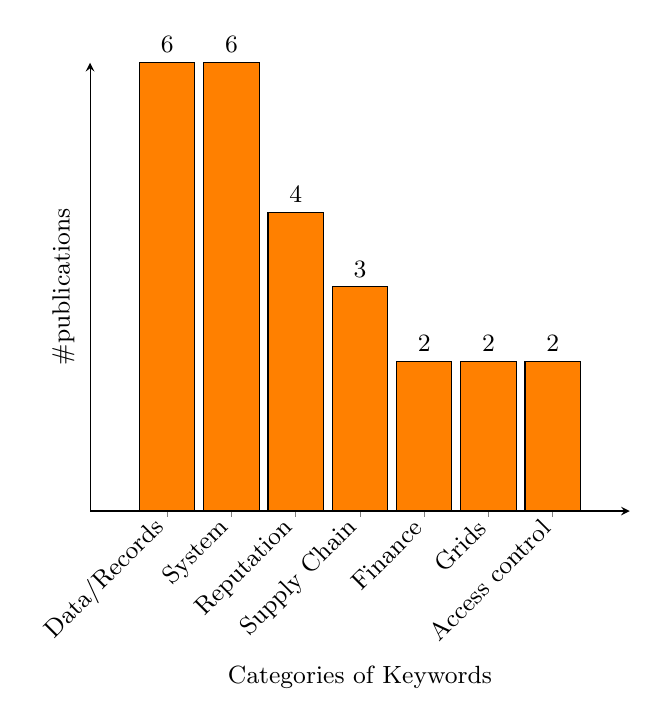
\begin{tikzpicture}[font=\small]
    \begin{axis}[
      ybar,
      bar width=20pt,
      xlabel={Categories of Keywords},
      ylabel={\#publications},
      ymin=0,
      ytick=\empty,
      xtick=data,
      axis x line=bottom,
      axis y line=left,
      enlarge x limits=0.2,
      symbolic x coords={Data/Records,System,Reputation,Supply Chain,Finance,Grids,Access control},
      nodes near coords,
      xticklabel style={rotate=45,anchor=east},
    ]
      \addplot[fill=orange] coordinates {
        (Data/Records,6)
        (System,6)
        (Reputation,4)
        (Supply Chain,3)
        (Finance,2)
        (Grids,2)
        (Access control,2)
      };
    \end{axis}
  \end{tikzpicture}

%______________________________________________________________________

\clearpage
\subsection{Content-based Information}
\label{subsec:ContentBasedInformation}
\textcolor{red}{\textbf{[TO DO]}}
\subsubsection{RQ6: Authors}
\subsubsection{RQ7: Contribution}
\subsubsection{RQ8: Reason/Problems}
\subsubsection{RQ9: Implementation Process}
\subsubsection{RQ10: Conclusion}

